\documentclass{report}

%%%%%%%%%%%%%%%%%%%%%%%%%%%%%%%%%
% PACKAGE IMPORTS
%%%%%%%%%%%%%%%%%%%%%%%%%%%%%%%%%


\usepackage[tmargin=2cm,rmargin=1in,lmargin=1in,margin=0.85in,bmargin=2cm,footskip=.2in]{geometry}
\usepackage{amsmath,amsfonts,amsthm,amssymb,mathtools}
\usepackage{bookmark}
\usepackage{enumitem}
\usepackage{hyperref,theoremref}
\hypersetup{
	pdftitle={Analysis 2 Class Notes},
	colorlinks=true, linkcolor=doc!90,
	bookmarksnumbered=true,
	bookmarksopen=true
}
\usepackage[most,many,breakable]{tcolorbox}
\usepackage{xcolor}
\usepackage{graphicx}
\graphicspath{ {./images/} }
\usepackage{varwidth}
\usepackage{varwidth}
\usepackage{etoolbox}
%\usepackage{authblk}
\usepackage{nameref}
\usepackage{multicol,array}
\usepackage{tikz-cd}
\usepackage{cancel}
\usepackage{pgfplots}
\pgfplotsset{compat=newest}
\usepgfplotslibrary{patchplots}
\usepackage{anyfontsize}
\usepackage{sectsty}
%\usepackage{import}
%\usepackage{xifthen}
%\usepackage{pdfpages}
%\usepackage{transparent}


%%%%%%%%%%%%%%%%%%%%%%%%%%%%%%
% SELF MADE COLORS
%%%%%%%%%%%%%%%%%%%%%%%%%%%%%%

\usetikzlibrary{ shapes.geometric }
\usetikzlibrary{calc}
\usepackage{anyfontsize}

\definecolor{myg}{RGB}{56, 140, 70}
\definecolor{myb}{RGB}{45, 111, 177}
\definecolor{myr}{RGB}{199, 68, 64}
\definecolor{mytheorembg}{HTML}{F2F2F9}
\definecolor{mytheoremfr}{HTML}{00007B}
\definecolor{myexamplebg}{HTML}{F2FBF8}
\definecolor{myexamplefr}{HTML}{88D6D1}
\definecolor{myexampleti}{HTML}{2A7F7F}
\definecolor{mydefinitbg}{HTML}{E5E5FF}
\definecolor{mydefinitfr}{HTML}{3F3FA3}
\definecolor{notesgreen}{RGB}{0,162,0}
\definecolor{myp}{RGB}{197, 92, 212}
\definecolor{mygr}{HTML}{2C3338}
\definecolor{myred}{RGB}{127,0,0}
\definecolor{myyellow}{RGB}{169,121,69}
\definecolor{OrangeRed}{HTML}{ED135A}
\definecolor{Dandelion}{HTML}{FDBC42}
\definecolor{light-gray}{gray}{0.95}
\definecolor{Emerald}{HTML}{00A99D}
\definecolor{RoyalBlue}{HTML}{0071BC}


%%%%%%%%%%%%%%%%%%%%%%%%%%%%
% TCOLORBOX SETUPS
%%%%%%%%%%%%%%%%%%%%%%%%%%%%

\setlength{\parindent}{1cm}
%================================
% THEOREM BOX
%================================

\tcbuselibrary{theorems,skins,hooks}
\newtcbtheorem[number within=section]{Theorem}{Theorem}
{%
	enhanced,
	breakable,
	colback = mytheorembg,
	frame hidden,
	boxrule = 0sp,
	borderline west = {2pt}{0pt}{mytheoremfr},
	sharp corners,
	detach title,
	before upper = \tcbtitle\par\smallskip,
	coltitle = mytheoremfr,
	fonttitle = \bfseries\sffamily,
	description font = \mdseries,
	separator sign none,
	segmentation style={solid, mytheoremfr},
}
{th}

\tcbuselibrary{theorems,skins,hooks}
\newtcbtheorem[number within=chapter]{theorem}{Theorem}
{%
	enhanced,
	breakable,
	colback = mytheorembg,
	frame hidden,
	boxrule = 0sp,
	borderline west = {2pt}{0pt}{mytheoremfr},
	sharp corners,
	detach title,
	before upper = \tcbtitle\par\smallskip,
	coltitle = mytheoremfr,
	fonttitle = \bfseries\sffamily,
	description font = \mdseries,
	separator sign none,
	segmentation style={solid, mytheoremfr},
}
{th}


\tcbuselibrary{theorems,skins,hooks}
\newtcolorbox{Theoremcon}
{%
	enhanced
	,breakable
	,colback = mytheorembg
	,frame hidden
	,boxrule = 0sp
	,borderline west = {2pt}{0pt}{mytheoremfr}
	,sharp corners
	,description font = \mdseries
	,separator sign none
}


%================================
% Corollery
%================================
\tcbuselibrary{theorems,skins,hooks}
\newtcbtheorem[number within=section]{corolary}{Corollary}
{%
	enhanced
	,breakable
	,colback = myp!10
	,frame hidden
	,boxrule = 0sp
	,borderline west = {2pt}{0pt}{myp!85!black}
	,sharp corners
	,detach title
	,before upper = \tcbtitle\par\smallskip
	,coltitle = myp!85!black
	,fonttitle = \bfseries\sffamily
	,description font = \mdseries
	,separator sign none
	,segmentation style={solid, myp!85!black}
}
{th}
\tcbuselibrary{theorems,skins,hooks}
\newtcbtheorem[number within=chapter]{corollary}{Corollary}
{%
	enhanced
	,breakable
	,colback = myp!10
	,frame hidden
	,boxrule = 0sp
	,borderline west = {2pt}{0pt}{myp!85!black}
	,sharp corners
	,detach title
	,before upper = \tcbtitle\par\smallskip
	,coltitle = myp!85!black
	,fonttitle = \bfseries\sffamily
	,description font = \mdseries
	,separator sign none
	,segmentation style={solid, myp!85!black}
}
{th}

%================================
% CLAIM
%================================

\tcbuselibrary{theorems,skins,hooks}
\newtcbtheorem[number within=section]{claim}{Claim}
{%
	enhanced
	,breakable
	,colback = myg!10
	,frame hidden
	,boxrule = 0sp
	,borderline west = {2pt}{0pt}{myg}
	,sharp corners
	,detach title
	,before upper = \tcbtitle\par\smallskip
	,coltitle = myg!85!black
	,fonttitle = \bfseries\sffamily
	,description font = \mdseries
	,separator sign none
	,segmentation style={solid, myg!85!black}
}
{th}


\newtcbtheorem[number within=chapter]{Claim}{Claim}
{%
	enhanced
	,breakable
	,colback = myg!10
	,frame hidden
	,boxrule = 0sp
	,borderline west = {2pt}{0pt}{myg}
	,sharp corners
	,detach title
	,before upper = \tcbtitle\par\smallskip
	,coltitle = myg!85!black
	,fonttitle = \bfseries\sffamily
	,description font = \mdseries
	,separator sign none
	,segmentation style={solid, myg!85!black}
}
{th}

%================================
% EXAMPLE BOX
%================================

\newtcbtheorem[number within=section]{Example}{Example}
{%
	colback = myexamplebg
	,breakable
	,colframe = myexamplefr
	,coltitle = myexampleti
	,boxrule = 1pt
	,sharp corners
	,detach title
	,before upper=\tcbtitle\par\smallskip
	,fonttitle = \bfseries
	,description font = \mdseries
	,separator sign none
	,description delimiters parenthesis
}
{ex}

\newtcbtheorem[number within=chapter]{example}{Example}
{%
	colback = myexamplebg
	,breakable
	,colframe = myexamplefr
	,coltitle = myexampleti
	,boxrule = 1pt
	,sharp corners
	,detach title
	,before upper=\tcbtitle\par\smallskip
	,fonttitle = \bfseries
	,description font = \mdseries
	,separator sign none
	,description delimiters parenthesis
}
{ex}

%================================
% DEFINITION BOX
%================================

\newtcbtheorem[number within=section]{Definition}{Definition}{enhanced,
	before skip=2mm,after skip=2mm, colback=red!5,colframe=red!80!black,boxrule=0.5mm,
	attach boxed title to top left={xshift=1cm,yshift*=1mm-\tcboxedtitleheight}, varwidth boxed title*=-3cm,
	boxed title style={frame code={
					\path[fill=tcbcolback]
					([yshift=-1mm,xshift=-1mm]frame.north west)
					arc[start angle=0,end angle=180,radius=1mm]
					([yshift=-1mm,xshift=1mm]frame.north east)
					arc[start angle=180,end angle=0,radius=1mm];
					\path[left color=tcbcolback!60!black,right color=tcbcolback!60!black,
						middle color=tcbcolback!80!black]
					([xshift=-2mm]frame.north west) -- ([xshift=2mm]frame.north east)
					[rounded corners=1mm]-- ([xshift=1mm,yshift=-1mm]frame.north east)
					-- (frame.south east) -- (frame.south west)
					-- ([xshift=-1mm,yshift=-1mm]frame.north west)
					[sharp corners]-- cycle;
				},interior engine=empty,
		},
	fonttitle=\bfseries,
	title={#2},#1}{def}
\newtcbtheorem[number within=chapter]{definition}{Definition}{enhanced,
	before skip=2mm,after skip=2mm, colback=red!5,colframe=red!80!black,boxrule=0.5mm,
	attach boxed title to top left={xshift=1cm,yshift*=1mm-\tcboxedtitleheight}, varwidth boxed title*=-3cm,
	boxed title style={frame code={
					\path[fill=tcbcolback]
					([yshift=-1mm,xshift=-1mm]frame.north west)
					arc[start angle=0,end angle=180,radius=1mm]
					([yshift=-1mm,xshift=1mm]frame.north east)
					arc[start angle=180,end angle=0,radius=1mm];
					\path[left color=tcbcolback!60!black,right color=tcbcolback!60!black,
						middle color=tcbcolback!80!black]
					([xshift=-2mm]frame.north west) -- ([xshift=2mm]frame.north east)
					[rounded corners=1mm]-- ([xshift=1mm,yshift=-1mm]frame.north east)
					-- (frame.south east) -- (frame.south west)
					-- ([xshift=-1mm,yshift=-1mm]frame.north west)
					[sharp corners]-- cycle;
				},interior engine=empty,
		},
	fonttitle=\bfseries,
	title={#2},#1}{def}


%================================
% OPEN QUESTION BOX
%================================

\newtcbtheorem[number within=section]{open}{Open Question}{enhanced,
	before skip=2mm,after skip=2mm, colback=myp!5,colframe=myp!80!black,boxrule=0.5mm,
	attach boxed title to top left={xshift=1cm,yshift*=1mm-\tcboxedtitleheight}, varwidth boxed title*=-3cm,
	boxed title style={frame code={
			\path[fill=tcbcolback]
			([yshift=-1mm,xshift=-1mm]frame.north west)
			arc[start angle=0,end angle=180,radius=1mm]
			([yshift=-1mm,xshift=1mm]frame.north east)
			arc[start angle=180,end angle=0,radius=1mm];
			\path[left color=tcbcolback!60!black,right color=tcbcolback!60!black,
			middle color=tcbcolback!80!black]
			([xshift=-2mm]frame.north west) -- ([xshift=2mm]frame.north east)
			[rounded corners=1mm]-- ([xshift=1mm,yshift=-1mm]frame.north east)
			-- (frame.south east) -- (frame.south west)
			-- ([xshift=-1mm,yshift=-1mm]frame.north west)
			[sharp corners]-- cycle;
		},interior engine=empty,
	},
	fonttitle=\bfseries,
	title={#2},#1}{def}
\newtcbtheorem[number within=chapter]{Open}{Open Question}{enhanced,
	before skip=2mm,after skip=2mm, colback=myp!5,colframe=myp!80!black,boxrule=0.5mm,
	attach boxed title to top left={xshift=1cm,yshift*=1mm-\tcboxedtitleheight}, varwidth boxed title*=-3cm,
	boxed title style={frame code={
			\path[fill=tcbcolback]
			([yshift=-1mm,xshift=-1mm]frame.north west)
			arc[start angle=0,end angle=180,radius=1mm]
			([yshift=-1mm,xshift=1mm]frame.north east)
			arc[start angle=180,end angle=0,radius=1mm];
			\path[left color=tcbcolback!60!black,right color=tcbcolback!60!black,
			middle color=tcbcolback!80!black]
			([xshift=-2mm]frame.north west) -- ([xshift=2mm]frame.north east)
			[rounded corners=1mm]-- ([xshift=1mm,yshift=-1mm]frame.north east)
			-- (frame.south east) -- (frame.south west)
			-- ([xshift=-1mm,yshift=-1mm]frame.north west)
			[sharp corners]-- cycle;
		},interior engine=empty,
	},
	fonttitle=\bfseries,
	title={#2},#1}{def}



%================================
% EXERCISE BOX
%================================

\makeatletter
\newtcbtheorem{question}{Question}{enhanced,
	breakable,
	colback=white,
	colframe=myb!80!black,
	attach boxed title to top left={yshift*=-\tcboxedtitleheight},
	fonttitle=\bfseries,
	title={#2},
	boxed title size=title,
	boxed title style={%
			sharp corners,
			rounded corners=northwest,
			colback=tcbcolframe,
			boxrule=0pt,
		},
	underlay boxed title={%
			\path[fill=tcbcolframe] (title.south west)--(title.south east)
			to[out=0, in=180] ([xshift=5mm]title.east)--
			(title.center-|frame.east)
			[rounded corners=\kvtcb@arc] |-
			(frame.north) -| cycle;
		},
	#1
}{def}
\makeatother

%================================
% SOLUTION BOX
%================================

\makeatletter
\newtcolorbox{solution}{enhanced,
	breakable,
	colback=white,
	colframe=myg!80!black,
	attach boxed title to top left={yshift*=-\tcboxedtitleheight},
	title=Solution,
	boxed title size=title,
	boxed title style={%
			sharp corners,
			rounded corners=northwest,
			colback=tcbcolframe,
			boxrule=0pt,
		},
	underlay boxed title={%
			\path[fill=tcbcolframe] (title.south west)--(title.south east)
			to[out=0, in=180] ([xshift=5mm]title.east)--
			(title.center-|frame.east)
			[rounded corners=\kvtcb@arc] |-
			(frame.north) -| cycle;
		},
}
\makeatother

%================================
% Question BOX
%================================

\makeatletter
\newtcbtheorem{qstion}{Question}{enhanced,
	breakable,
	colback=white,
	colframe=mygr,
	attach boxed title to top left={yshift*=-\tcboxedtitleheight},
	fonttitle=\bfseries,
	title={#2},
	boxed title size=title,
	boxed title style={%
			sharp corners,
			rounded corners=northwest,
			colback=tcbcolframe,
			boxrule=0pt,
		},
	underlay boxed title={%
			\path[fill=tcbcolframe] (title.south west)--(title.south east)
			to[out=0, in=180] ([xshift=5mm]title.east)--
			(title.center-|frame.east)
			[rounded corners=\kvtcb@arc] |-
			(frame.north) -| cycle;
		},
	#1
}{def}
\makeatother

\newtcbtheorem[number within=chapter]{wconc}{Wrong Concept}{
	breakable,
	enhanced,
	colback=white,
	colframe=myr,
	arc=0pt,
	outer arc=0pt,
	fonttitle=\bfseries\sffamily\large,
	colbacktitle=myr,
	attach boxed title to top left={},
	boxed title style={
			enhanced,
			skin=enhancedfirst jigsaw,
			arc=3pt,
			bottom=0pt,
			interior style={fill=myr}
		},
	#1
}{def}



%================================
% NOTE BOX
%================================

\usetikzlibrary{arrows,calc,shadows.blur}
\tcbuselibrary{skins}
\newtcolorbox{note}[1][]{%
	enhanced jigsaw,
	colback=gray!20!white,%
	colframe=gray!80!black,
	size=small,
	boxrule=1pt,
	title=\textbf{Note:-},
	halign title=flush center,
	coltitle=black,
	breakable,
	drop shadow=black!50!white,
	attach boxed title to top left={xshift=1cm,yshift=-\tcboxedtitleheight/2,yshifttext=-\tcboxedtitleheight/2},
	minipage boxed title=1.5cm,
	boxed title style={%
			colback=white,
			size=fbox,
			boxrule=1pt,
			boxsep=2pt,
			underlay={%
					\coordinate (dotA) at ($(interior.west) + (-0.5pt,0)$);
					\coordinate (dotB) at ($(interior.east) + (0.5pt,0)$);
					\begin{scope}
						\clip (interior.north west) rectangle ([xshift=3ex]interior.east);
						\filldraw [white, blur shadow={shadow opacity=60, shadow yshift=-.75ex}, rounded corners=2pt] (interior.north west) rectangle (interior.south east);
					\end{scope}
					\begin{scope}[gray!80!black]
						\fill (dotA) circle (2pt);
						\fill (dotB) circle (2pt);
					\end{scope}
				},
		},
	#1,
}

%%%%%%%%%%%%%%%%%%%%%%%%%%%%%%
% SELF MADE COMMANDS
%%%%%%%%%%%%%%%%%%%%%%%%%%%%%%

%% The environments which are appears in pairs one of them is for the chapters which have sections whose environment name starts with small letter and the other is for chapters which do not have sections whose environment name starts with capital letter. In the short command for the latter I used the letter 'c' to represent it should be use if it is not under a section


\NewDocumentCommand{\EqM}{ m O{black} m}{%
	\tikz[remember picture, baseline, anchor=base] 
	\node[inner sep=0pt, outer sep=3pt, text=#2] (#1) {%
		\ensuremath{#3}%
	};    
}



\newcommand{\thm}[3][]{\begin{Theorem}{#2}{#1}#3\end{Theorem}}
\newcommand{\thmc}[3][]{\begin{theorem}{#2}{#1}#3\end{theorem}}
\newcommand{\cor}[3][]{\begin{corolary}{#2}{#1}#3\end{corolary}}
\newcommand{\corc}[3][]{\begin{corollary}{#2}{#1}#3\end{corollary}}
\newcommand{\clm}[3][]{\begin{claim}{#2}{#1}#3\end{claim}}
\newcommand{\wc}[3][]{\begin{wconc}{#2}{#1}\setlength{\parindent}{1cm}#3\end{wconc}}
\newcommand{\thmcon}[1]{\begin{Theoremcon}{#1}\end{Theoremcon}}
\newcommand{\ex}[3][]{\begin{Example}{#2}{#1}#3\end{Example}}
\newcommand{\exc}[3][]{\begin{example}{#2}{#1}#3\end{example}}
\newcommand{\dfn}[3][]{\begin{Definition}[colbacktitle=red!75!black]{#2}{#1}#3\end{Definition}}
\newcommand{\dfnc}[3][]{\begin{definition}[colbacktitle=red!75!black]{#2}{#1}#3\end{definition}}
\newcommand{\opn}[3][]{\begin{open}[colbacktitle=myp!75!black]{#2}{#1}#3\end{open}}
\newcommand{\opnc}[3][]{\begin{Open}[colbacktitle=myp!75!black]{#2}{#1}#3\end{Open}}
\newcommand{\qs}[3][]{\begin{question}{#2}{#1}#3\end{question}}
\newcommand{\pf}[2]{\begin{myproof}[#1]#2\end{myproof}}
\newcommand{\nt}[1]{\begin{note}#1\end{note}}

\newcommand*\circled[1]{\tikz[baseline=(char.base)]{
		\node[shape=circle,draw,inner sep=1pt] (char) {#1};}}
\newcommand\getcurrentref[1]{%
	\ifnumequal{\value{#1}}{0}
	{??}
	{\the\value{#1}}%
}
\newcommand{\getCurrentSectionNumber}{\getcurrentref{section}}
\newenvironment{myproof}[1][\proofname]{%
	\proof[\bfseries #1: ]%
}{\endproof}
\newcounter{mylabelcounter}

\makeatletter
\newcommand{\setword}[2]{%
	\phantomsection
	#1\def\@currentlabel{\unexpanded{#1}}\label{#2}%
}
\makeatother




\tikzset{
	symbol/.style={
			draw=none,
			every to/.append style={
					edge node={node [sloped, allow upside down, auto=false]{$#1$}}}
		}
}


%%%%%%%%%%%%%%%%%%%%%%%%%%%%%%%%%%%%%%%%%%%
% TABLE OF CONTENTS 1
%%%%%%%%%%%%%%%%%%%%%%%%%%%%%%%%%%%%%%%%%%%

%\usepackage{framed}
%\usepackage{titletoc}
%\usepackage{etoolbox}
%\usepackage{lmodern}


%\patchcmd{\tableofcontents}{\contentsname}{\sffamily\contentsname}{}{}

%\renewenvironment{leftbar}
%{\def\FrameCommand{\hspace{6em}%
%		{\color{myyellow}\vrule width 2pt depth 6pt}\hspace{1em}}%
%	\MakeFramed{\parshape 1 0cm \dimexpr\textwidth-6em\relax\FrameRestore}\vskip2pt%
%}
%{\endMakeFramed}

%\titlecontents{chapter}
%[0em]{\vspace*{2\baselineskip}}
%{\parbox{4.5em}{%
%		\hfill\Huge\sffamily\bfseries\color{myred}\thecontentspage}%
%	\vspace*{-2.3\baselineskip}\leftbar\textsc{\small\chaptername~\thecontentslabel}\\\sffamily}
%{}{\endleftbar}
%\titlecontents{section}
%[8.4em]
%{\sffamily\contentslabel{3em}}{}{}
%{\hspace{0.5em}\nobreak\itshape\color{myred}\contentspage}
%\titlecontents{subsection}
%[8.4em]
%{\sffamily\contentslabel{3em}}{}{}  
%{\hspace{0.5em}\nobreak\itshape\color{myred}\contentspage}



%%%%%%%%%%%%%%%%%%%%%%%%%%%%%%%%%%%%%%%%%%%
% TABLE OF CONTENTS 2
%%%%%%%%%%%%%%%%%%%%%%%%%%%%%%%%%%%%%%%%%%%

\usepackage{tikz}
\definecolor{doc}{RGB}{0,60,110}
\usepackage{titletoc}
\contentsmargin{0cm}
\titlecontents{chapter}[3.7pc]
{\addvspace{30pt}%
	\begin{tikzpicture}[remember picture, overlay]%
		\draw[fill=doc!60,draw=doc!60] (-7,-.1) rectangle (-0.7,.5);%
		\pgftext[left,x=-3.6cm,y=0.2cm]{\color{white}\Large\sc\bfseries Chapter\ \thecontentslabel};%
	\end{tikzpicture}\color{doc!60}\large\sc\bfseries}%
{}
{}
{\;\titlerule\;\large\sc\bfseries Page \thecontentspage
	\begin{tikzpicture}[remember picture, overlay]
		\draw[fill=doc!60,draw=doc!60] (2pt,0) rectangle (4,0.1pt);
	\end{tikzpicture}}%
\titlecontents{section}[3.7pc]
{\addvspace{2pt}}
{\contentslabel[\thecontentslabel]{2pc}}
{}
{\hfill\small \thecontentspage}
[]
\titlecontents*{subsection}[3.7pc]
{\addvspace{-1pt}\small}
{}
{}
{\ --- \small\thecontentspage}
[ \textbullet\ ][]

\makeatletter
\renewcommand{\tableofcontents}{%
	\chapter*{%
	  \vspace*{-20\p@}%
	  \begin{tikzpicture}[remember picture, overlay]%
		  \pgftext[right,x=15cm,y=0.2cm]{\color{doc!60}\Huge\sc\bfseries \contentsname};%
		  \draw[fill=doc!60,draw=doc!60] (13,-.75) rectangle (20,1);%
		  \clip (13,-.75) rectangle (20,1);
		  \pgftext[right,x=15cm,y=0.2cm]{\color{white}\Huge\sc\bfseries \contentsname};%
	  \end{tikzpicture}}%
	\@starttoc{toc}}
\makeatother

\newcommand{\mytitlea}[4]{
	\begin{tikzpicture}[remember picture,overlay]
		%%%%%%%%%%%%%%%%%%%% Background %%%%%%%%%%%%%%%%%%%%%%%%
		\fill[orange] (current page.south west) rectangle (current page.north east);
		
		
		
		
		%%%%%%%%%%%%%%%%%%%% Background Polygon %%%%%%%%%%%%%%%%%%%%
		
		\foreach \i in {2.5,...,22}
		{
			\node[rounded corners,orange!60,draw,regular polygon,regular polygon sides=6, minimum size=\i cm,ultra thick] at ($(current page.west)+(2.5,-5)$) {} ;
		}
		
		\foreach \i in {0.5,...,22}
		{
			\node[rounded corners,orange!60,draw,regular polygon,regular polygon sides=6, minimum size=\i cm,ultra thick] at ($(current page.north west)+(2.5,0)$) {} ;
		}
		
		\foreach \i in {0.5,...,22}
		{
			\node[rounded corners,orange!90,draw,regular polygon,regular polygon sides=6, minimum size=\i cm,ultra thick] at ($(current page.north east)+(0,-9.5)$) {} ;
		}
		
		
		\foreach \i in {21,...,6}
		{
			\node[orange!85,rounded corners,draw,regular polygon,regular polygon sides=6, minimum size=\i cm,ultra thick] at ($(current page.south east)+(-0.2,-0.45)$) {} ;
		}
		
		
		%%%%%%%%%%%%%%%%%%%% Title of the Report %%%%%%%%%%%%%%%%%%%% 
		\node[left,black,minimum width=0.625*\paperwidth,minimum height=3cm, rounded corners] at ($(current page.north east)+(0,-9.5)$)
		{
			{\fontsize{25}{30} \selectfont \bfseries #1}
		};
		
		%%%%%%%%%%%%%%%%%%%% Subtitle %%%%%%%%%%%%%%%%%%%% 
		\node[left,black,minimum width=0.625*\paperwidth,minimum height=2cm, rounded corners] at ($(current page.north east)+(0,-11)$)
		{
			{\huge \textit{#2}}
		};
		
		%%%%%%%%%%%%%%%%%%%% Author Name %%%%%%%%%%%%%%%%%%%% 
		\node[left,black,minimum width=0.625*\paperwidth,minimum height=2cm, rounded corners] at ($(current page.north east)+(0,-13)$)
		{
			{\Large \textsc{#3}}
		};
		
		%%%%%%%%%%%%%%%%%%%% Year %%%%%%%%%%%%%%%%%%%% 
		\node[rounded corners,fill=orange!70,text =black,regular polygon,regular polygon sides=6, minimum size=2.5 cm,inner sep=0,ultra thick] at ($(current page.west)+(2.5,-5)$) {\LARGE \bfseries #4};
		
	\end{tikzpicture}
}
\newcommand{\mytitleb}[4]{\begin{tikzpicture}[overlay,remember picture]
		
		% Background color
		\fill[
		black!2]
		(current page.south west) rectangle (current page.north east);
		
		% Rectangles
		\shade[
		left color=Dandelion, 
		right color=Dandelion!40,
		transform canvas ={rotate around ={45:($(current page.north west)+(0,-6)$)}}] 
		($(current page.north west)+(0,-6)$) rectangle ++(9,1.5);
		
		\shade[
		left color=lightgray,
		right color=lightgray!50,
		rounded corners=0.75cm,
		transform canvas ={rotate around ={45:($(current page.north west)+(.5,-10)$)}}]
		($(current page.north west)+(0.5,-10)$) rectangle ++(15,1.5);
		
		\shade[
		left color=lightgray,
		rounded corners=0.3cm,
		transform canvas ={rotate around ={45:($(current page.north west)+(.5,-10)$)}}] ($(current page.north west)+(1.5,-9.55)$) rectangle ++(7,.6);
		
		\shade[
		left color=orange!80,
		right color=orange!60,
		rounded corners=0.4cm,
		transform canvas ={rotate around ={45:($(current page.north)+(-1.5,-3)$)}}]
		($(current page.north)+(-1.5,-3)$) rectangle ++(9,0.8);
		
		\shade[
		left color=red!80,
		right color=red!80,
		rounded corners=0.9cm,
		transform canvas ={rotate around ={45:($(current page.north)+(-3,-8)$)}}] ($(current page.north)+(-3,-8)$) rectangle ++(15,1.8);
		
		\shade[
		left color=orange,
		right color=Dandelion,
		rounded corners=0.9cm,
		transform canvas ={rotate around ={45:($(current page.north west)+(4,-15.5)$)}}]
		($(current page.north west)+(4,-15.5)$) rectangle ++(30,1.8);
		
		\shade[
		left color=RoyalBlue,
		right color=Emerald,
		rounded corners=0.75cm,
		transform canvas ={rotate around ={45:($(current page.north west)+(13,-10)$)}}]
		($(current page.north west)+(13,-10)$) rectangle ++(15,1.5);
		
		\shade[
		left color=lightgray,
		rounded corners=0.3cm,
		transform canvas ={rotate around ={45:($(current page.north west)+(18,-8)$)}}]
		($(current page.north west)+(18,-8)$) rectangle ++(15,0.6);
		
		\shade[
		left color=lightgray,
		rounded corners=0.4cm,
		transform canvas ={rotate around ={45:($(current page.north west)+(19,-5.65)$)}}]
		($(current page.north west)+(19,-5.65)$) rectangle ++(15,0.8);
		
		\shade[
		left color=OrangeRed,
		right color=red!80,
		rounded corners=0.6cm,
		transform canvas ={rotate around ={45:($(current page.north west)+(20,-9)$)}}] 
		($(current page.north west)+(20,-9)$) rectangle ++(14,1.2);
		
		% Year
		\draw[ultra thick,gray]
		($(current page.center)+(5,2)$) -- ++(0,-3cm) 
		node[
		midway,
		left=0.25cm,
		text width=5cm,
		align=right,
		black!75
		]
		{
			{\fontsize{25}{30} \selectfont \bf  Lecture\\[10pt] Notes}
		} 
		node[
		midway,
		right=0.25cm,
		text width=6cm,
		align=left,
		orange]
		{
			{\fontsize{72}{86.4} \selectfont #4}
		};
		
		% Title
		\node[align=center] at ($(current page.center)+(0,-5)$) 
		{
			{\fontsize{60}{72} \selectfont {{#1}}} \\[1cm]
			{\fontsize{16}{19.2} \selectfont \textcolor{orange}{ \bf #2}}\\[3pt]
			#3};
\end{tikzpicture}
}
\newcommand{\Qed}{\begin{flushright}\qed\end{flushright}}
\newcommand{\parinn}{\setlength{\parindent}{1cm}}
\newcommand{\parinf}{\setlength{\parindent}{0cm}}
\newcommand{\del}[2]{\frac{\partial #1}{\partial #2}}
\newcommand{\Del}[3]{\frac{\partial^{#1} #2}{\partial^{#1} #3}}
\newcommand{\deld}[2]{\dfrac{\partial #1}{\partial #2}}
\newcommand{\Deld}[3]{\dfrac{\partial^{#1} #2}{\partial^{#1} #3}}
\newcommand{\uin}{\mathbin{\rotatebox[origin=c]{90}{$\in$}}}
\newcommand{\usubset}{\mathbin{\rotatebox[origin=c]{90}{$\subset$}}}
\newcommand{\lt}{\left}
\newcommand{\rt}{\right}
\newcommand{\exs}{\exists}
\newcommand{\st}{\strut}
\newcommand{\dps}[1]{\displaystyle{#1}}
\newcommand{\la}{\langle}
\newcommand{\ra}{\rangle}
\newenvironment{solution}
{\textit{\textbf{Solution:}} 
}
{ 
	\hfill $\blacksquare$
	
	\vspace{1cm}
}
\newcommand{\sol}[1]{\begin{solution}#1\end{solution}}
\newcommand{\solve}[1]{\setlength{\parindent}{0cm}\textbf{\textit{Solution: }}\setlength{\parindent}{1cm}#1 \Qed}
\newcommand{\mat}[1]{\left[\begin{matrix}#1\end{matrix}\right]}
\newcommand\numberthis{\addtocounter{equation}{1}\tag{\theequation}}
\newcommand{\handout}[3]{
	\noindent
	\begin{center}
		\framebox{
			\vbox{
				\hbox to 6.5in { {\bf Complexity Theory I } \hfill Jan -- May, 2023 }
				\vspace{4mm}
				\hbox to 6.5in { {\Large \hfill #1  \hfill} }
				\vspace{2mm}
				\hbox to 6.5in { {\em #2 \hfill #3} }
			}
		}
	\end{center}
	\vspace*{4mm}
}

\newcommand{\lecture}[3]{\handout{Lecture #1}{Lecturer: #2}{Scribe:	#3}}
	

\newcommand{\ov}[1]{\overline{#1}}
\newcommand{\thmref}[1]{\hyperref[#1]{Theorem \ref{#1}}}
%---------------------------------------
% BlackBoard Math Fonts :-
%---------------------------------------

%Captital Letters
\newcommand{\bbA}{\mathbb{A}}	\newcommand{\bbB}{\mathbb{B}}
\newcommand{\bbC}{\mathbb{C}}	\newcommand{\bbD}{\mathbb{D}}
\newcommand{\bbE}{\mathbb{E}}	\newcommand{\bbF}{\mathbb{F}}
\newcommand{\bbG}{\mathbb{G}}	\newcommand{\bbH}{\mathbb{H}}
\newcommand{\bbI}{\mathbb{I}}	\newcommand{\bbJ}{\mathbb{J}}
\newcommand{\bbK}{\mathbb{K}}	\newcommand{\bbL}{\mathbb{L}}
\newcommand{\bbM}{\mathbb{M}}	\newcommand{\bbN}{\mathbb{N}}
\newcommand{\bbO}{\mathbb{O}}	\newcommand{\bbP}{\mathbb{P}}
\newcommand{\bbQ}{\mathbb{Q}}	\newcommand{\bbR}{\mathbb{R}}
\newcommand{\bbS}{\mathbb{S}}	\newcommand{\bbT}{\mathbb{T}}
\newcommand{\bbU}{\mathbb{U}}	\newcommand{\bbV}{\mathbb{V}}
\newcommand{\bbW}{\mathbb{W}}	\newcommand{\bbX}{\mathbb{X}}
\newcommand{\bbY}{\mathbb{Y}}	\newcommand{\bbZ}{\mathbb{Z}}

%---------------------------------------
% MathCal Fonts :-
%---------------------------------------

%Captital Letters
\newcommand{\mcA}{\mathcal{A}}	\newcommand{\mcB}{\mathcal{B}}
\newcommand{\mcC}{\mathcal{C}}	\newcommand{\mcD}{\mathcal{D}}
\newcommand{\mcE}{\mathcal{E}}	\newcommand{\mcF}{\mathcal{F}}
\newcommand{\mcG}{\mathcal{G}}	\newcommand{\mcH}{\mathcal{H}}
\newcommand{\mcI}{\mathcal{I}}	\newcommand{\mcJ}{\mathcal{J}}
\newcommand{\mcK}{\mathcal{K}}	\newcommand{\mcL}{\mathcal{L}}
\newcommand{\mcM}{\mathcal{M}}	\newcommand{\mcN}{\mathcal{N}}
\newcommand{\mcO}{\mathcal{O}}	\newcommand{\mcP}{\mathcal{P}}
\newcommand{\mcQ}{\mathcal{Q}}	\newcommand{\mcR}{\mathcal{R}}
\newcommand{\mcS}{\mathcal{S}}	\newcommand{\mcT}{\mathcal{T}}
\newcommand{\mcU}{\mathcal{U}}	\newcommand{\mcV}{\mathcal{V}}
\newcommand{\mcW}{\mathcal{W}}	\newcommand{\mcX}{\mathcal{X}}
\newcommand{\mcY}{\mathcal{Y}}	\newcommand{\mcZ}{\mathcal{Z}}



%---------------------------------------
% Bold Math Fonts :-
%---------------------------------------

%Captital Letters
\newcommand{\bmA}{\boldsymbol{A}}	\newcommand{\bmB}{\boldsymbol{B}}
\newcommand{\bmC}{\boldsymbol{C}}	\newcommand{\bmD}{\boldsymbol{D}}
\newcommand{\bmE}{\boldsymbol{E}}	\newcommand{\bmF}{\boldsymbol{F}}
\newcommand{\bmG}{\boldsymbol{G}}	\newcommand{\bmH}{\boldsymbol{H}}
\newcommand{\bmI}{\boldsymbol{I}}	\newcommand{\bmJ}{\boldsymbol{J}}
\newcommand{\bmK}{\boldsymbol{K}}	\newcommand{\bmL}{\boldsymbol{L}}
\newcommand{\bmM}{\boldsymbol{M}}	\newcommand{\bmN}{\boldsymbol{N}}
\newcommand{\bmO}{\boldsymbol{O}}	\newcommand{\bmP}{\boldsymbol{P}}
\newcommand{\bmQ}{\boldsymbol{Q}}	\newcommand{\bmR}{\boldsymbol{R}}
\newcommand{\bmS}{\boldsymbol{S}}	\newcommand{\bmT}{\boldsymbol{T}}
\newcommand{\bmU}{\boldsymbol{U}}	\newcommand{\bmV}{\boldsymbol{V}}
\newcommand{\bmW}{\boldsymbol{W}}	\newcommand{\bmX}{\boldsymbol{X}}
\newcommand{\bmY}{\boldsymbol{Y}}	\newcommand{\bmZ}{\boldsymbol{Z}}
%Small Letters
\newcommand{\bma}{\boldsymbol{a}}	\newcommand{\bmb}{\boldsymbol{b}}
\newcommand{\bmc}{\boldsymbol{c}}	\newcommand{\bmd}{\boldsymbol{d}}
\newcommand{\bme}{\boldsymbol{e}}	\newcommand{\bmf}{\boldsymbol{f}}
\newcommand{\bmg}{\boldsymbol{g}}	\newcommand{\bmh}{\boldsymbol{h}}
\newcommand{\bmi}{\boldsymbol{i}}	\newcommand{\bmj}{\boldsymbol{j}}
\newcommand{\bmk}{\boldsymbol{k}}	\newcommand{\bml}{\boldsymbol{l}}
\newcommand{\bmm}{\boldsymbol{m}}	\newcommand{\bmn}{\boldsymbol{n}}
\newcommand{\bmo}{\boldsymbol{o}}	\newcommand{\bmp}{\boldsymbol{p}}
\newcommand{\bmq}{\boldsymbol{q}}	\newcommand{\bmr}{\boldsymbol{r}}
\newcommand{\bms}{\boldsymbol{s}}	\newcommand{\bmt}{\boldsymbol{t}}
\newcommand{\bmu}{\boldsymbol{u}}	\newcommand{\bmv}{\boldsymbol{v}}
\newcommand{\bmw}{\boldsymbol{w}}	\newcommand{\bmx}{\boldsymbol{x}}
\newcommand{\bmy}{\boldsymbol{y}}	\newcommand{\bmz}{\boldsymbol{z}}

%---------------------------------------
% Scr Math Fonts :-
%---------------------------------------

\newcommand{\sA}{{\mathscr{A}}}   \newcommand{\sB}{{\mathscr{B}}}
\newcommand{\sC}{{\mathscr{C}}}   \newcommand{\sD}{{\mathscr{D}}}
\newcommand{\sE}{{\mathscr{E}}}   \newcommand{\sF}{{\mathscr{F}}}
\newcommand{\sG}{{\mathscr{G}}}   \newcommand{\sH}{{\mathscr{H}}}
\newcommand{\sI}{{\mathscr{I}}}   \newcommand{\sJ}{{\mathscr{J}}}
\newcommand{\sK}{{\mathscr{K}}}   \newcommand{\sL}{{\mathscr{L}}}
\newcommand{\sM}{{\mathscr{M}}}   \newcommand{\sN}{{\mathscr{N}}}
\newcommand{\sO}{{\mathscr{O}}}   \newcommand{\sP}{{\mathscr{P}}}
\newcommand{\sQ}{{\mathscr{Q}}}   \newcommand{\sR}{{\mathscr{R}}}
\newcommand{\sS}{{\mathscr{S}}}   \newcommand{\sT}{{\mathscr{T}}}
\newcommand{\sU}{{\mathscr{U}}}   \newcommand{\sV}{{\mathscr{V}}}
\newcommand{\sW}{{\mathscr{W}}}   \newcommand{\sX}{{\mathscr{X}}}
\newcommand{\sY}{{\mathscr{Y}}}   \newcommand{\sZ}{{\mathscr{Z}}}


%---------------------------------------
% Math Fraktur Font
%---------------------------------------

%Captital Letters
\newcommand{\mfA}{\mathfrak{A}}	\newcommand{\mfB}{\mathfrak{B}}
\newcommand{\mfC}{\mathfrak{C}}	\newcommand{\mfD}{\mathfrak{D}}
\newcommand{\mfE}{\mathfrak{E}}	\newcommand{\mfF}{\mathfrak{F}}
\newcommand{\mfG}{\mathfrak{G}}	\newcommand{\mfH}{\mathfrak{H}}
\newcommand{\mfI}{\mathfrak{I}}	\newcommand{\mfJ}{\mathfrak{J}}
\newcommand{\mfK}{\mathfrak{K}}	\newcommand{\mfL}{\mathfrak{L}}
\newcommand{\mfM}{\mathfrak{M}}	\newcommand{\mfN}{\mathfrak{N}}
\newcommand{\mfO}{\mathfrak{O}}	\newcommand{\mfP}{\mathfrak{P}}
\newcommand{\mfQ}{\mathfrak{Q}}	\newcommand{\mfR}{\mathfrak{R}}
\newcommand{\mfS}{\mathfrak{S}}	\newcommand{\mfT}{\mathfrak{T}}
\newcommand{\mfU}{\mathfrak{U}}	\newcommand{\mfV}{\mathfrak{V}}
\newcommand{\mfW}{\mathfrak{W}}	\newcommand{\mfX}{\mathfrak{X}}
\newcommand{\mfY}{\mathfrak{Y}}	\newcommand{\mfZ}{\mathfrak{Z}}
%Small Letters
\newcommand{\mfa}{\mathfrak{a}}	\newcommand{\mfb}{\mathfrak{b}}
\newcommand{\mfc}{\mathfrak{c}}	\newcommand{\mfd}{\mathfrak{d}}
\newcommand{\mfe}{\mathfrak{e}}	\newcommand{\mff}{\mathfrak{f}}
\newcommand{\mfg}{\mathfrak{g}}	\newcommand{\mfh}{\mathfrak{h}}
\newcommand{\mfi}{\mathfrak{i}}	\newcommand{\mfj}{\mathfrak{j}}
\newcommand{\mfk}{\mathfrak{k}}	\newcommand{\mfl}{\mathfrak{l}}
\newcommand{\mfm}{\mathfrak{m}}	\newcommand{\mfn}{\mathfrak{n}}
\newcommand{\mfo}{\mathfrak{o}}	\newcommand{\mfp}{\mathfrak{p}}
\newcommand{\mfq}{\mathfrak{q}}	\newcommand{\mfr}{\mathfrak{r}}
\newcommand{\mfs}{\mathfrak{s}}	\newcommand{\mft}{\mathfrak{t}}
\newcommand{\mfu}{\mathfrak{u}}	\newcommand{\mfv}{\mathfrak{v}}
\newcommand{\mfw}{\mathfrak{w}}	\newcommand{\mfx}{\mathfrak{x}}
\newcommand{\mfy}{\mathfrak{y}}	\newcommand{\mfz}{\mathfrak{z}}

%---------------------------------------
% Bar
%---------------------------------------

%Captital Letters
\newcommand{\barA}{\overline{A}}	\newcommand{\barB}{\overline{B}}
\newcommand{\barC}{\overline{C}}	\newcommand{\barD}{\overline{D}}
\newcommand{\barE}{\overline{E}}	\newcommand{\barF}{\overline{F}}
\newcommand{\barG}{\overline{G}}	\newcommand{\barH}{\overline{H}}
\newcommand{\barI}{\overline{I}}	\newcommand{\barJ}{\overline{J}}
\newcommand{\barK}{\overline{K}}	\newcommand{\barL}{\overline{L}}
\newcommand{\barM}{\overline{M}}	\newcommand{\barN}{\overline{N}}
\newcommand{\barO}{\overline{O}}	\newcommand{\barP}{\overline{P}}
\newcommand{\barQ}{\overline{Q}}	\newcommand{\barR}{\overline{R}}
\newcommand{\barS}{\overline{S}}	\newcommand{\barT}{\overline{T}}
\newcommand{\barU}{\overline{U}}	\newcommand{\barV}{\overline{V}}
\newcommand{\barW}{\overline{W}}	\newcommand{\barX}{\overline{X}}
\newcommand{\barY}{\overline{Y}}	\newcommand{\barZ}{\overline{Z}}
%Small Letters
\newcommand{\bara}{\overline{a}}	\newcommand{\barb}{\overline{b}}
\newcommand{\barc}{\overline{c}}	\newcommand{\bard}{\overline{d}}
\newcommand{\bare}{\overline{e}}	\newcommand{\barf}{\overline{f}}
\newcommand{\barg}{\overline{g}}	\newcommand{\barh}{\overline{h}}
\newcommand{\bari}{\overline{i}}	\newcommand{\barj}{\overline{j}}
\newcommand{\bark}{\overline{k}}	\newcommand{\barl}{\overline{l}}
\newcommand{\barm}{\overline{m}}	\newcommand{\barn}{\overline{n}}
\newcommand{\baro}{\overline{o}}	\newcommand{\barp}{\overline{p}}
\newcommand{\barq}{\overline{q}}	\newcommand{\barr}{\overline{r}}
\newcommand{\bars}{\overline{s}}	\newcommand{\bart}{\overline{t}}
\newcommand{\baru}{\overline{u}}	\newcommand{\barv}{\overline{v}}
\newcommand{\barw}{\overline{w}}	\newcommand{\barx}{\overline{x}}
\newcommand{\bary}{\overline{y}}	\newcommand{\barz}{\overline{z}}

%---------------------------------------
% Greek Letters:-
%---------------------------------------
\newcommand{\eps}{\epsilon}
\newcommand{\veps}{\varepsilon}
\newcommand{\lm}{\lambda}
\newcommand{\Lm}{\Lambda}
\newcommand{\gm}{\gamma}
\newcommand{\Gm}{\Gamma}
\newcommand{\vph}{\varphi}
\newcommand{\ph}{\phi}

\title{\Huge{Analysis 2 Lecture Notes}\\ \hspace{4cm}-- Upendra Kulkarni}
\author{\huge{Soham Chatterjee}}
\date{}

\begin{document}
\maketitle
\newpage% or \cleardoublepage
% \pdfbookmark[<level>]{<title>}{<dest>}
\pagebreak

\vspace*{5cm}

\begin{center}
	\textbf{Abstract}
\end{center}

This is the lecture notes scribed by me. If you find any mistakes in the notes please email me at \url{sohamc@cmi.ac.in}. 

The whole course is taken by Prof. Upendra Kulkarni, online. If you want the lectures then you can find them in \href{https://youtube.com/playlist?list=PL8I7rVYxS9smyQemVlU10yF9F37ZQN38P}{this link}. Sir mainly followed Prof. Pramath Sastry's Notes (\url{https://www.cmi.ac.in/~pramath/teaching.html#ANA2}). You can find all the assignments problems in the following  \href{https://drive.google.com/drive/folders/1dODMladIJ1f4BfMXVxoU5_YkfmWU8v4q?usp=share_link}{drive link}. Through out the course the books we followed is  Principles of Mathematical Analysis by Walter Rudin. 

\pagebreak
\chapter{Constrained Optimizations and Lagrange Multipliers}
\parinf

\textbf{\textit{Example: }}Optimize $f(x,y)y^2-x^2$ subject to the constraint $h(x,y)=x^2+y^2=1$
\parinn

\begin{center}
	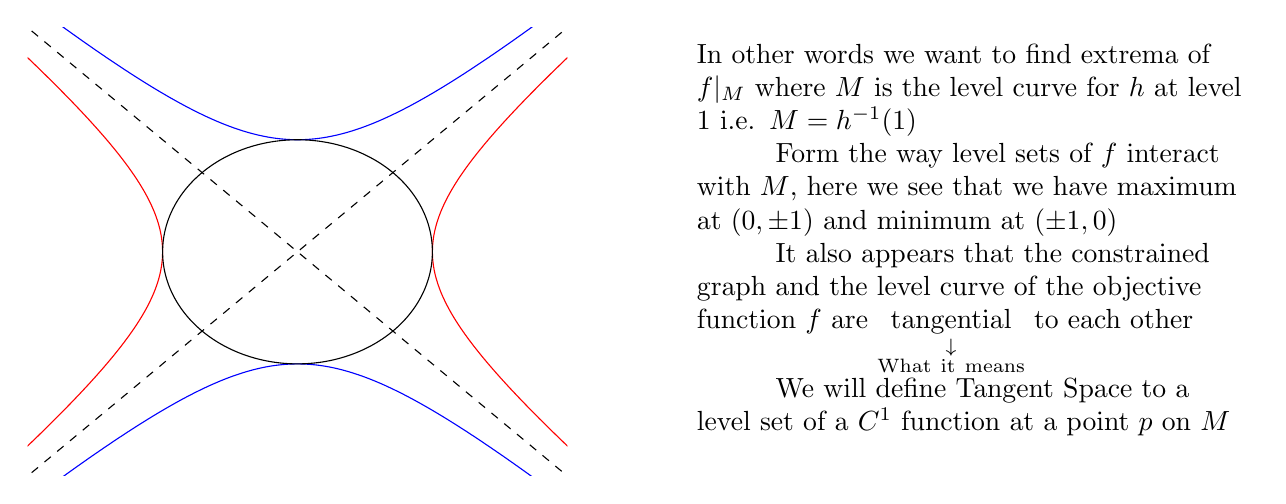
\begin{tikzpicture}
		
		\begin{axis}[xmin=-2,xmax=2, ymin=-2, ymax=2,
			restrict x to domain=-10:10, hide axis]% remove crossing lines at t=90 and t=270
			\addplot[red, variable=t,domain=0:360,samples=200] ({sec(t)}, {tan(t)});
			\addplot[blue,variable=t,domain=0:360,samples=200] ({tan(t)}, {sec(t)});
			\addplot[dashed]{x};
			\addplot[dashed]{-x};
			\addplot[variable=t,domain=0:360,samples=200]  ({cos(t)}, {sin(t)}) ;
		\end{axis}
	\node[text width=7cm, xshift=12cm,yshift=3cm]{\parindent=1cm In other words we want to find extrema of $f|_M$ where $M$ is the level curve for $h$ at level 1 i.e. $M=h^{-1}(1)$
	
Form the way level sets of $f$ interact with $M$, here we see that we have maximum at $(0,\pm 1)$ and minimum at $(\pm 1,0)$

It also appears that the constrained graph and the level curve of the objective function $f$ are $\underset{ \substack{ \downarrow \\ \text{What it means} } }{\text{tangential}}$ to each other

We will define Tangent Space to a level set of a $C^1$ function at a point $p$ on $M$
};
	\end{tikzpicture}
\end{center}
\section{Tangent Space}
\dfn{Tangent Space}{Tangent Space to a hypersurface $M=f^{-1}(c)$ in $\bbR^n$ where $f:(\text{Open }U\subset \bbR^n)\to \bbR$ is a $C^1$ function and $c\in \bbR$ at a point $p\in M$ is a subspace of $\bbR^n$ defined to be $$T_pM=\ker (f'(p))=\{v\in\bbR^n\mid f'(p)(v)=0\}=\{v\in \bbR^n\mid \nabla f(p)\cdot v=0\}$$}
Geometric tangent space considering to our mental image = $T_pM+p=$ Shift $T_pM$ by vector $p$. Likewise define Normal Space to be the set of vectors orthogonal to $T_pM$ i.e. $T_pM^{\perp}$

\begin{center}
	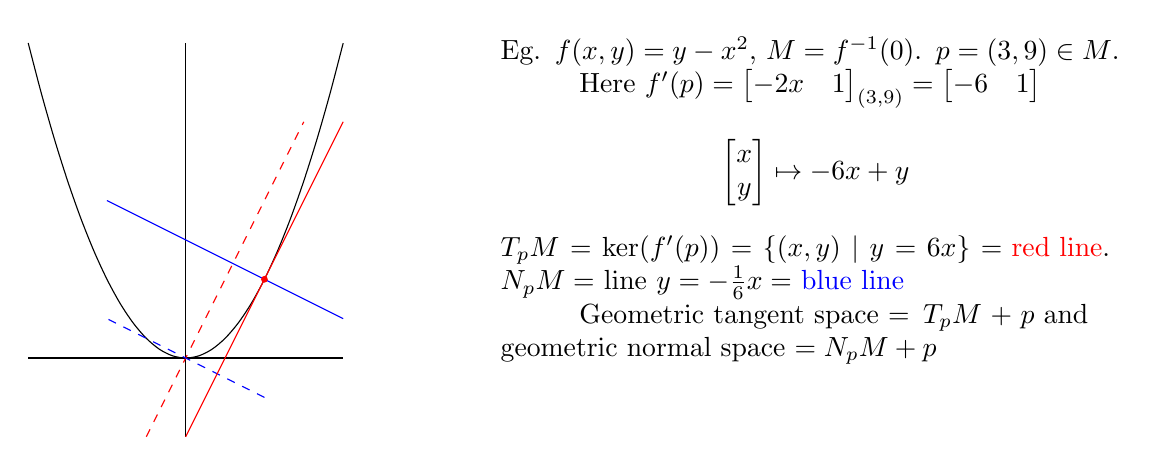
\begin{tikzpicture}
		\draw[domain=-2:2, smooth, variable=\x] plot ({\x}, {\x*\x});
		\draw (-2,0) -- (2,0);
		\draw (0,4) -- (0,-1);
		\draw[red,dashed] (-0.5,-1) -- (1.5,3);
		\draw[blue,dashed] (1,-0.5) -- (-1,0.5);
		\draw[red] (0,-1) -- (2,3);
		\draw[blue] (2,0.5) -- (-1,2);
		\filldraw[red] (1,1) circle (1pt);
		\node[text width=8cm, xshift=8cm,yshift=2cm]{\parindent=1cm 
		Eg. $f(x,y)=y-x^2$, $M=f^{-1}(0)$. $p=(3,9)\in M$. 
		
		Here $f'(p)=\mat{-2x & 1}_{(3,9)}=\mat{-6& 1}$ $$\mat{x \\ y} \mapsto -6x+y$$ $T_pM=\ker(f'(p))=\{ (x,y)\mid y=6x\}=$ \textcolor{red}{red line}. $N_pM= $ line $y=-\frac16 x =$ \textcolor{blue}{blue line}
		
		Geometric tangent space $=T_pM+p$ and geometric normal space $=N_pM+p$
	};
	\end{tikzpicture}
\end{center}
\section{Lagrange Multiplier}
Let $U$ be open in $\bbR^n$. $f:U\to \bbR$ objective function and $h:U\to \bbR$ constraint function. Want to find extrema of $f$ restricted to the level set $M=\{x\in U\mid h(x)=c\}=h^{-1}(c)$ for $c\in\bbR$

$f|_M$ has local maxima at $p\in M$ means for some $W\subset  U$,  $f(p)\geq f(x)\ \forall \ x\in W\cap M$
\dfn{$C^1$ Path and Velocity Vector}{A $C^1$ path centered at $p\in U$ in $U\subset \bbR^n$ is a $C^1$ map $\gm:(-\veps,\veps)\to U$ where $0\mapsto p$. We call $\gm'(0)=$ velocity of $\gm$ at 0}
\thm[lagmult]{Lagrange Multiplier}{
Let $U$ be open in $\bbR^n$. $f:U\to \bbR$, $h:U\to \bbR$. Let $f,h$ are $C^1$ functions. Let $M=h^{-1}(c)$. If $h'(p)\neq 0$ and $f|_M$ has  a local extrema  at $p\in M$  then  $\exs!\lm\in \bbR$ such that $$\nabla f(p)=\lm \nabla h(p)$$
}
\begin{proof}
Consider paths on level set $M=h^{-1}(c)$ i.e. \begin{center}
	\begin{tikzcd}[column sep={3em},/tikz/column 1/.style={column sep=0},/tikz/column 3/.style={column sep=0em}]
	\gm: &  (-\veps,\veps) \arrow[r] \arrow[rdd]&  M &=h^{-1}(c)\\[-8mm]
	 &  & \cap & \\[-8mm]
	 && U \arrow[r, "h"] & \bbR
\end{tikzcd}
\end{center}
Then $h=\gm(t)=c$ $\forall\ t\in (-\veps,\veps)$. Hence by Chain Rule $$h'(p)\gm'(0)=\nabla h(p)\cdot \gm'(0)=0$$ i.e. $\{\text{velocity vectors of all paths }\gm\text{ on }M\text{ centered at }p\}\subset T_pM$\parinf

\textbf{\textit{Key Fact: }}When $h'(p)\neq 0$ we have equality! Proof of this fact uses \hyperref[th:implicit]{Implicit Function Theorem}\parinn

Now let's recall the objective function $f$ and recall that $p$ is assured to be a local max/min. If $\gm$ is a $C^1$ curve on $M$ then in particular $f|_{\text{image}(\gm)}$ also has a max/min at $p$. Therefore $$0=(f\circ \gm)'(o)=\nabla f(p)\cdot \gm'(0)$$i.e. $\nabla f$ is orthogonal to velocity vectors to all curves centered at $p$. 

By claim $\nabla f(p)\perp T_pM$, we already  say $\nabla h(p)\perp T_pM$. We know $\nabla h(p)\neq 0$ by assumption. Hence $\exs! \lm$ such that $\nabla f(p)=\lm \nabla h(p)$
\end{proof}

\section{Some Examples for Applications}
\begin{enumerate}[label=(\roman*)]
	\item $f(x,y)=y^2-h^2$ and $h(x,y)=x^2+y^2$, $c=1$. Therefore $M=h^{-1}(1)=$ Unit Circle
	
	Suppose $p=\mat{a\\ b}$ is an extremum of $f|_M$ $$\nabla f(p)=\mat{-2x\\ 2y}_{(a,b)} = \mat{-2a\\ 2b}\qquad \nabla h(p)=\mat{2x\\ 2y}_{(a,b)} = \mat{2a\\ 2b}$$ We know that $\exs ! \lm \in \bbR$ such that $$\mat{-2a\\ 2b}=\lm \mat{2a\\ 2b}$$ This is not possible unless one of $a,b$ os 0. Therefore \begin{center}
		\begin{tabular}{lcl}
			$a=0$ & $\implies $ &$b=\pm 1$ and $\lm=1$\\
			$b=0$ & $\implies$ & $a=\pm 1$ and $\lm=-1$
		\end{tabular}
	\end{center}
\item $f(x,y)=y$ is subject to constraint $h(x,y)=y-g(x)=0$ where $g:\bbR\to \bbR$ is some $C^1$ function. This is equivalent to finding extrema of $y=g(x)$ as in school

Suppose  $p=\mat{a\\ b}$ gives an extremum $$\nabla f(p)=\mat{0\\ 1}= \lm \nabla h(p)=\lm \mat{-g'(a)\\ 1}$$i.e. $1=\lm\implies 0=-\lm g'(a)\implies g'(a)=0$ as expected
\item $f(x,y)=x^2$ subject to $h(x,y)=y=0$ $$\nabla f=\mat{2x\\ 0}=\lm\nabla h=\mat{0\\ 1}\implies \lm =0, x=0$$
\nt{If we instead take $h(x,y)=y^2$, then we get $(,xy)=(0,0)$ but $\lm$ arbitrary}
\item $f(x,y)=xy$ subject to $h(x,y)=\frac{x^2}{9}+\frac{y^2}{4}=1$

$$\nabla f=\mat{y\\ x} = \lm \nabla h=\lm \mat{\frac{2x}{9}\\ \frac{y}{2}}$$ Therefore $$y=\frac{2x}{9}\lm, \quad x=\frac{y}{2}\lm, \quad \frac{x^2}{9}+\frac{y^2}{4}=1$$ 

$\lm=\pm 3$. Find extrema. As constraint = ellipse, a compact set, evaluating $f$ as candidates is enough to find max and min.
\item Find the points on the sphere $x^2+y^2+z^2=9$ closest/furthest from $(a,b,c)\to$ arbitrary point in $\bbR^3$

$f(x,y,z)=(x-a)^2+(y-b)^2+(z-c)^2$ and $h(x,y,z)=x^2+y^2+z^2=9$. Complete this and see that geometrically obvious solution emerge 
\end{enumerate}

Next we will prove \hyperref[th:invthm]{Inverse Function Theorem} and \hyperref[th:implicit]{Implicit Function Theorem} and come back to justify the claim. In fact we will then be able to prove the general version of Lagrange Multiplier Method i.e. with multiple constraints

\section{Generalized Lagrange Multiplier}
\thm[genlagmult]{Generalized Lagrange Multiplier}{$U$ open $\subset \bbR^n=\bbR^{d+m}$ want to find extrema of objective function $f:U\to \bbR$ subject to constraint $h=c$ for a $C^1$ function: $U\to \bbR^m$ where $c\in \bbR^m$  i.e. we want to find extreme of $f|_{M=h^{1}(c)}$
}\parinf

\textbf{\textit{Key Assumption: }}$\forall\ x\in M$, $h'(x)$ is surjective i.e. $h'(x):\bbR^{d+m}\to \bbR^m$. (So $\ker(h'(x))$ has $\dim d$. Recall we called $\ker(h'(x))=T_xM$)

Suppose $f|_M$ has a local extremum at $p\in M$ Then $\exs!$ real numbers $\lm_1,\lm_2,\dots,\lm_m$ such that $$\nabla f(p)=\lm_1\nabla h_1(p)+\cdots+\lm_n\nabla h_n(p)$$where $h(p)=\mat{h_1(p) & \cdots & h_m(p)}^T\in \bbR^m$

\parinn
\begin{proof}
	we will show that \begin{enumerate}[label=\bfseries\tiny\protect\circled{\small\arabic*}]
		\item  $\nabla f(p)\perp T_pM$
		\item Any vector $\perp T_pM$ is a linear combination of $\nabla h_i(p)$
	\end{enumerate}
These are the steps. 
\begin{enumerate}[label=\bfseries\tiny\protect\circled{\small\arabic*}]
	\item Let $v\in T_pM=\ker (f'(p))$. By \href{https://drive.google.com/file/d/11OCy_upvhLy8mH0jCKwFbXqzEX3FBT8Z/view?usp=share_link}{HW4 Problem} $v$ can be represented by some curve based at $p$ i.e. we can find a $C^1$ curve $\gm:(-\veps,\veps)\to M\subset U$ where $0\mapsto p$ such that $\gm'(0)=v$. 
	
	As we have an extremum of $f|M$ at $p$ it is also an extreme point for $(-\veps,\veps)\xrightarrow{\gm}M\xrightarrow{f}\bbR$. So by 1-Variable Calculus $(f\circ\gm)'(0)=0$ i.e. $f'(p)\gm'(0)=0$ i.e. $\nabla f(p)\cdot v=0$
	
	\item For every curve $\gm$ as above $h\circ \gm=$ constant. Therefore $h'(p)\gm'(0)=0$ i.e. $\nabla h'(p)\cdot v=0$ $$h'(p)=\mat{ \del{h_1}{x_1}(p)   & \cdots & \del{h_1}{x_n}(p) \\ \vdots & \ddots & \vdots \\ \del{h_m}{x_1}(p)   & \cdots & \del{h_m}{x_n}(p)  }=\mat{\nabla h_1(p)^T \\ \vdots \\ \nabla h_m(p)^T}=\mat{\nabla h_1(p) & \cdots & \nabla h_m(p)}^T$$ So $$\nabla h_1(p)\cdot v=0,\dots , \nabla h_m(p)\cdot v=0$$Therefore $\underset{\substack{ m\text{ linearly} \\ \text{independent} \\ \text{vectors}  }}{\underbrace{\nabla h_i(p)}}\perp \underset{\substack{ \dim n-m \\ =d }}{\underbrace{T_pM}}$. Everything is in $\bbR^n=\bbR^{m+d}$. $\therefore (T_pM)^{\perp}$ has $\nabla h_1(p),\dots, \nabla h_m(p)$ as a basis. i.e. \circled{2} is proved
\end{enumerate}
\end{proof}

\chapter{Implicit Function Theorem}
\textbf{Notation: }For $n>m$ let $n=m+d$. Write points of $\bbR^n=\bbR^d\times \bbR^m$ as $(x,y)$ where $x\in \bbR^d,$ $y\in \bbR^m$
\thmc[implicit]{Implicit Function Theorem}{
Let $U$ open in $\bbR^{d+m}$. $\Phi:U\to \bbR^m$ is a $C^1$ map such that $\Phi'(p)$ is surjective (which means columns of the $m\times (d+m)$ matrix of $\Phi'(p)$ span $\bbR^m$). WLOG suppose the last $m$ columns of $\Phi'(p) $ are linearly independent and hence span $\bbR^m$ i.e. the $m\times m$ matrix ``$\lt.\deld{\Phi}{y}\rt|_p=\mat{D_{d+1}\Phi(p) & \cdots & D_{d+m}\Phi(p)} $" is invertible. Then \begin{enumerate}
	\item $\exs$ a neighorhood $W$ of $a$ in $\bbR^d$ and a unique $C^1$ map $W\xrightarrow{f}\bbR^m$ such that $\begin{rcases}
		f(a)=b, (x,f(x))\in U\ \forall \ x\in W\text{ and}\\
		\Phi(x,f(x))=c\ \forall \ x\in W
	\end{rcases}$ i.e. $f$ is an implicit solution to the equation $\Phi(x,y)=c$
\item One can calculate $f'(x)$ by ``Implicit Differentiation"
\end{enumerate}
}
To understand this, first examine two cases:
\begin{itemize}
	\item When $\Phi$ is a linear map given by a matrix $A$. Here we are solving the equation $A\mat{x\\ y}=c$
	\item $d=m=1$ i.e. $n=2$ $\Phi(x,y)=x^2+y^2-1$, solving $\Phi(x,y)=0=c$. When $\lt.\deld{\Phi}{y}\rt|_{p=(a,b)}\neq 0$ we can locally solve for $y$ in terms of $x$ near $p$. $$D\Phi=\lt.\mat{\del{\Phi}{x} & \del{\Phi}{y}}\rt|_{(a,b)}=\mat{2a & 2b}$$ $2b=0$ at $(\pm 1,0)$
\end{itemize}
\begin{proof}
	We will choose $W$ later. Define \begin{center}
		\begin{tikzcd}
			U \arrow[r, "\psi"] & \bbR^{d+m}\\
			(x,y)\arrow[r, maps to] & (x, \Phi(x,y))
		\end{tikzcd}
	\end{center}
Note $\psi'$ has the matrix $\mat{I & O\\ \del{\Phi}{x} & \del{\Phi}{y}}$. This is nonsingular in a neighborhood of $p$. So by \hyperref[th:invthm]{Inverse Function Theorem} $\psi$ is invertible with $C^1$ inverse in a neighborhood $V$ of $p$
\begin{center}
	\begin{tikzcd}
		V \arrow[r] & \psi(V) \arrow[l]\\[-8mm]
		(a,b)\arrow[r, maps to] & (a,c)\\[-8mm]
		(x,y)\arrow[r, maps to] & (x,\Phi(x,y))\\[-8mm]
		(u,\alpha(u,v)) & (u,v) \arrow[l, maps to]
	\end{tikzcd}
\end{center}Definition of $\alpha(u,v)$ defined on $\psi(V)$. This tells us $\alpha(a,c)=b$. Whenever $\Phi(x,y)=c$ i.e. $$(x,y)\xrightarrow{\Phi}(x,c)\xrightarrow{\psi^{-1}}(x,\alpha(x,c))=(x,y)$$ i.e. $y=\alpha(x,c)$ and $\Phi(x,\alpha(x,c))=c$

So we are forced to define $f(x)=\alpha(x,c)$. But what should be the domain of this function $f$ i.e. what should we take $W$ to be. 

\begin{center}
	$(a,c)\in \psi(V)$ is open $\supset$ $\lt( \text{\begin{tabular}{c}
		open ball $W$ \\ around $a$ in $\bbR^d$
	\end{tabular}} \rt)\times \{c\} $
\end{center}

Now for any $x\in W$ we know $(x,c)\in \psi(V)$ i.e. $(x,\alpha(x,c))\in V$ so we define $f:W\to \bbR^m$ where $f(x)=\alpha(x,c)$ and we have derived the function. Now $\phi^{-1}$ is $C^1$ and $\alpha$ is component of $\phi^{-1}$ so all components of $\phi^{-1}$ is also $C^1$. hence $f$ is $C^1$

Uniqueness of $f$ is not true in general for arbitrary $W$. $\Phi(x,y)=x^2+y^2,\ c=1$. In $W=W_1\sqcup W_2$ $$f(x)=\begin{cases}
	\sqrt{1-x^2} & x\in W_1 \qquad[\text{is forced}]\\
	\sqrt{1-x^2} \text{ or }-\sqrt{1-x^2} & x\in W_2
\end{cases}$$. We have choice for $f$ on $W_2$. 

\textbf{If $W$ is connected, $f$ will be unique}. Eg. take $W$ to be a ball.  Suppose $g$ is another solution to $\Phi(x,y)=c$ i.e. $\Phi(x,g(x))=c$ for $x\in W$ and $g(a)=b$. Then consider the set $S=\{x\in W\mid f(x)=g(x)\}$. Show that this set is both closed (easy $S=(f-g)^{-1}(0)$) and open. 


Calculate derivative of $f$ using the fact that $\psi\circ \psi^{-1}=$ Identity and Chain Rule.
\end{proof}
\ex{Application of Implicit Function Theorem}{
\begin{enumerate}[label=(\roman*)]
	\item Linear map $\Phi:\bbR^{d+m}\to \bbR^m$ given by matrix $A$. Given $A\mat{a\\ b}=c$. Want to solve $A\mat{x\\ y}=c$
	
	$A=[P \mid Q]$ where $P$ is $m\times d$ and $Q$ is $m\times m$ and $Q$ is invertible. i.e. \begin{multline*}
		[P\mid Q]\mat{x\\ y}=c\iff [Q^{-1}P\mid I]\mat{x\\ y}=Q^{-1}c\iff Q^{-1}Px+y=Q^{-1}c\\
		\iff y=Q^{-1}c-Q^{-1}Px
	\end{multline*}
\item We can solve for $y$ in terms of $x$ near any $(a,b)$ on the unit circle when $\lt.\deld{\Phi}{y}\rt|_{(a,b)}\neq 0$. [This is mate when $b\neq 0$ i.e. at all points except $(\pm 1,0)$]. $$\lt.D\Phi\rt|_{(a,b)}=\mat{2a& 2b}$$ We can see directly 

\begin{center}
	$\begin{rcases}
		\text{when }b>0 & y=\sqrt{1-x^2}\\
		\text{when }b<0 & y=-\sqrt{1-x^2}
	\end{rcases}$ near (a,b) in fact $\forall\ x\in (-1,1)$
\end{center}
Similarly we can solve for $x$ in terms of $y$ when $\lt.\deld{\Phi}{x}\rt|_{(a,b)}=2a\neq 0$ This is true when $a\neq 0$
\end{enumerate}

}
\pagebreak
\textbf{\textit{Remark: }} Implicit Function Theorem gives a sufficient condition to be able to locally solve a system of linear equations \begin{center}
	$\begin{rcases}
		\Phi_1(x_1,\dots,x_d,y_1,\dots,y_m)=c_1\\
		\Phi_2(x_1,\dots,x_d,y_1,\dots,y_m)=c_1\\
		\qquad\vdots \qquad\qquad \vdots \qquad\qquad \vdots\\
		\Phi_m(x_1,\dots,x_d,y_1,\dots,y_m)=c_1
	\end{rcases}$\begin{tabular}{l}
	for $y_i$'s in terms of $x_i$'s \\
	locally near a given solution\\
	$y=b$ and $x=a$
\end{tabular}
\end{center}

\nt{
The condition of invertibility of submatrix of $\Phi$ is not necessary. Eg. $\Phi(x,y)=y-x^3$ near $(0,0)$ $$\lt.D\Phi\rt|_{(0,0)}=\lt. \mat{-3x^2 & 1}\rt|_{(0,0)}=\mat{0,1} \qquad \lt.\deld{\Phi}{x}\rt|{(0,0)}=0$$ but still we can solve for $x$ in terms of $y$: $x=\sqrt[3]{y}$ 
}

\end{document}
